\chapter{Resultados y discusión}
\label{ch:resultados}

En este capítulo se presentan los resultados obtenidos tras aplicar los distintos algoritmos de clasificación sobre los conjuntos de datos preparados en las fases anteriores. El objetivo principal es evaluar el rendimiento de cada modelo bajo diferentes escenarios y métricas, con el fin de identificar sus fortalezas y limitaciones en la detección de \textit{malware}.

\vspace{1em}

Para ello, se analizan tanto los experimentos realizados en el problema binario, donde se distingue entre \textit{software} malicioso y benigno, como en el problema multiclase, en el que se busca identificar el tipo específico de amenaza. Los clasificadores se evalúan considerando como métricas: la sensibilidad mínima y la precisión de los modelos.

\vspace{1em}

Asimismo, se discute la capacidad de generalización de cada modelo, observando las diferencias de rendimiento entre los conjuntos de entrenamiento y prueba, así como la influencia de la variabilidad introducida por el desbalanceo de clases. Con este análisis se pretende ofrecer una visión comparativa que facilite la elección del modelo más adecuado en un contexto práctico de detección de amenazas.

\newpage
\section{Clasificación binaria}
\label{sec:clas_binaria}

En primer lugar se expondrán los resultados obtenidos en clasificación binaria.

\subsection{Árboles de decisión}
\label{subsec:dt_bin}

La tabla \ref{tabla:dt_bin} muestra los resultados de la clasificación binaria utilizando el modelo \texttt{DecisionTreeClassifier}, evaluado en 10 ejecuciones distintas con diferentes estados.

\begin{table}[H]
	\centering
	\begin{tabular}{ |c|c|c|c|c| }
		\hline
		\rowcolor{LightCyan}
		 & \multicolumn{2}{c|}{Entrenamiento} & \multicolumn{2}{c|}{Generalización} \\
		\hline
		\rowcolor{LightCyan}
		Semilla & Acc & MS & Acc & MS \\
		\hline
		0    & \textbf{1.000} & \textbf{1.000} & \textit{0.951} & 0.942           \\
		1    & \textit{1.000} & \textit{1.000} & 0.944          & 0.935           \\
		2    & 1.000          & 1.000          & 0.942          & 0.935           \\
		3    & 1.000          & 1.000          & 0.948          & 0.938           \\
		4    & 1.000          & 1.000          & \textbf{0.953} & \textbf{0.946}  \\
		5    & 0.998          & 0.997          & 0.947          & 0.936           \\
		6    & 0.998          & 0.997          & 0.947          & 0.941           \\
		7    & 1.000          & 1.000          & 0.949          & \textit{0.946}  \\
		8    & 0.999          & 0.998          & 0.948          & 0.937           \\
		9    & 1.000          & 1.000          & 0.950          & 0.940           \\
		Mean & 0.999          & 0.999          & 0.948          & 0.940           \\
		STD  & 0.001          & 0.001          & 0.003          & 0.004           \\
		\hline
	\end{tabular}
	\caption{Resultados en entrenamiento y generalización para las distintas semillas en clasificación binaria con \texttt{DecisionTreeClassifier}.}
	\label{tabla:dt_bin}
\end{table}

Para el entrenamiento, la precisión (\textit{Acc}), la sensibilidad mínima (\textit{MS}) y el \textit{Valor-F1} alcanzan valores muy próximos a 1 en todas las ejecuciones. En cuanto al test, la precisión oscila entre 0.942 y 0.953, mientras que la sensibilidad mínima se sitúa entre 0.935 y 0.946.

\vspace{1em}

la figura \ref{fig:dt_bin} compara la distribución de los valores de \textit{accuracy} en entrenamiento y en test para el clasificador basado en árboles de decisión. Se observa que en entrenamiento son consistentemente cercanos a 1, sin apenas variabilidad, lo que indica que el modelo es capaz de ajustarse casi perfectamente a los datos de entrenamiento.

\newpage

En contraste, los valores en test muestran una ligera caída, con una variabilidad mayor que en entrenamiento. Esta diferencia refleja que el modelo generaliza de forma aceptable, aunque la brecha respecto al rendimiento en entrenamiento sugiere la existencia de cierto sobreajuste.

\vspace{1em}

El uso combinado de \texttt{violinplot} y \texttt{boxplot} permite apreciar tanto la concentración de los valores en torno a la media como la dispersión entre diferentes ejecuciones. En este caso, el test mantiene una distribución compacta, sin valores atípicos extremos, lo que aporta robustez a la evaluación del modelo.

\begin{figure}[H]
	\centering
	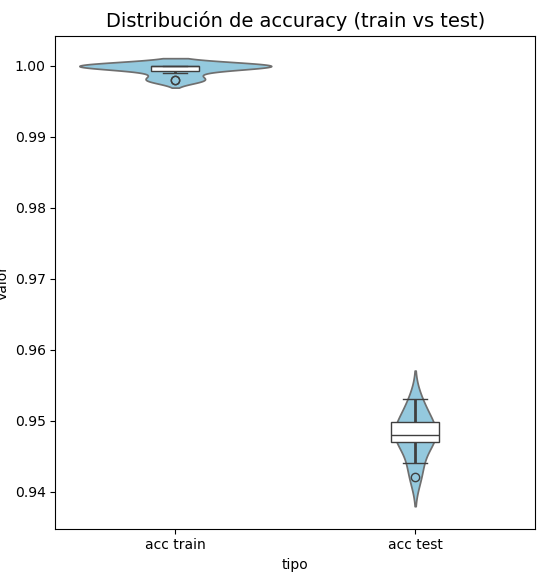
\includegraphics[width=1\linewidth]{Imagenes/dt_bin}
	\caption[\texttt{Boxplot} con \texttt{violinplot} para árboles de decisión]{\texttt{Boxplot} con \texttt{violinplot} para árboles de decisión.}
	\label{fig:dt_bin}
\end{figure}

\newpage
\subsection{\textit{Random forest}}
\label{subsec:rf_bin}

En la tabla \ref{tabla:rf_bin} se muestran los resultados de la clasificación binaria utilizando el modelo \texttt{RandomForestClassifier} para diferentes estados aleatorios.

\begin{table}[H]
	\centering
	\begin{tabular}{ |c|c|c|c|c| }
		\hline
		\rowcolor{LightCyan}
		 & \multicolumn{2}{c|}{Entrenamiento} & \multicolumn{2}{c|}{Generalización} \\
		\hline
		\rowcolor{LightCyan}
		 Semilla & Acc & MS & Acc & MS \\
		\hline
		0    & 0.980          & 0.928          & 0.939          & 0.524          \\
		1    & 0.980          & 0.929          & 0.939          & 0.500          \\
		2    & 0.980          & 0.927          & \textbf{0.941} & 0.429          \\
		3    & 0.979          & 0.923          & 0.939          & 0.444          \\
		4    & 0.982          & 0.931          & 0.939          & 0.500          \\
		5    & 0.980          & 0.929          & 0.937          & \textbf{0.609} \\
		6    & 0.978          & 0.920          & 0.938          & 0.550          \\
		7    & 0.980          & 0.929          & 0.939          & 0.562          \\
		8    & 0.982          & 0.934          & 0.938          & 0.489          \\
		9    & \textbf{0.989} & \textbf{0.956} & 0.936          & 0.400          \\
		Mean & 0.981          & 0.931          & 0.939          & 0.501          \\
		STD  & 0.003          & 0.010          & 0.001          & 0.064          \\
		\hline
	\end{tabular}
	\caption{Resultados en entrenamiento y generalización para las distintas semillas en clasificación binaria con \texttt{RandomForestClassifier}.}
	\label{tabla:rf_bin}
\end{table}

En el conjunto de entrenamiento, las métricas presentan valores altos y consistentes: la precisión oscila entre 0.978 y 0.989, la métrica de sensibilidad mínima entre 0.920 y 0.956.

\vspace{1em}

En el conjunto de prueba, la precisión mantiene valores muy estables alrededor de 0.936–0.941. La sensibilidad mínima muestra una mayor variabilidad, con valores que van desde 0.400 hasta 0.609.

\begin{figure}[H]
	\centering
	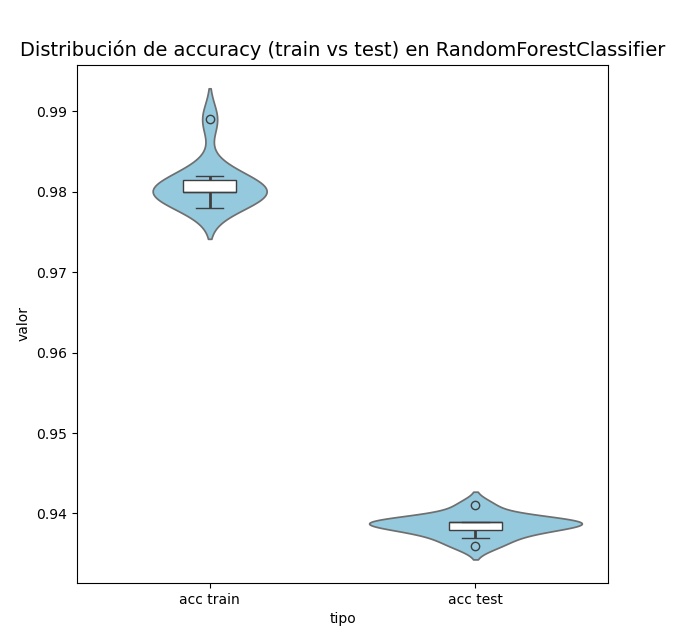
\includegraphics[width=1\linewidth]{Imagenes/rf_bin}
	\caption[\texttt{Boxplot} con \texttt{violinplot} para \texttt{RandomForestClassifier}]{\texttt{Boxplot} con \texttt{violinplot} para \texttt{RandomForestClassifier}.}
	\label{fig:rf_bin}
\end{figure}

El modelo muestra un rendimiento muy alto y consistente en precisión tanto en el entrenamiento como en el test. En la figura \ref{fig:rf_bin}, se observa que la distribución de \textit{accuracy} es estrecha, con valores muy concentrados en torno a 0.98 en entrenamiento y 0.94 en test, lo que indica estabilidad en ambas fases.

\newpage
Sin embargo, la métrica de sensibilidad mínima (\textit{MS}) introduce un matiz importante: aunque en entrenamiento se mantiene elevada con poca dispersión, en test presenta una gran variabilidad. El rango de valores oscila entre 0.400 y 0.609 según la semilla utilizada, lo que se traduce en distribuciones más amplias en los gráficos. Esto indica que, en algunos casos, el modelo no logra identificar de forma adecuada los ejemplos más difíciles de una de las clases, comprometiendo la robustez de la clasificación en escenarios concretos.

\subsection{\textit{K-NN}}
\label{subsec:knn_bin}

En la tabla \ref{tabla:knn_bin} se muestran los resultados obtenidos con el clasificador \texttt{KNeighborsClassifier} bajo diferentes semillas.

\begin{table}[H]
	\centering
	\begin{tabular}{ |c|c|c|c|c| }
		\hline
		\rowcolor{LightCyan}
		 & \multicolumn{2}{c|}{Entrenamiento} & \multicolumn{2}{c|}{Generalización} \\
		\hline
		\rowcolor{LightCyan}
		 Semilla & Acc & MS & Acc & MS \\
		\hline
		0    & 1.000          & 1.000          & 0.947          & 0.935          \\
		1    & 1.000          & 1.000          & 0.949          & 0.938          \\
		2    & 1.000          & 1.000          & 0.939          & 0.926          \\
		3    & 1.000          & 1.000          & 0.949          & 0.937          \\
		4    & 1.000          & 1.000          & 0.949          & 0.936          \\
		5    & 1.000          & 1.000          & 0.946          & 0.932          \\
		6    & 1.000          & 1.000          & 0.946          & 0.931          \\
		7    & 1.000          & 1.000          & 0.944          & 0.934          \\
		8    & 1.000          & 1.000          & 0.947          & 0.935          \\
		9    & \textbf{1.000} & \textbf{1.000} & \textbf{0.949} & \textbf{0.940} \\
		Mean & 1.000          & 1.000          & 0.947          & 0.934          \\
		STD  & 0.000          & 0.000          & 0.003          & 0.004          \\
		\hline
	\end{tabular}
	\caption{Resultados en entrenamiento y generalización para las distintas semillas en clasificación binaria con \texttt{KNeighborsClassifier}.}
	\label{tabla:knn_bin}
\end{table}

En la fase de entrenamiento, todas las semillas reportan valores de \textit{Acc} y \textit{MS} iguales a 1.000, lo que refleja una completa uniformidad en las métricas. La media confirma este comportamiento perfecto, con desviaciones estándar nulas en las tres métricas.

\newpage
En la fase de generalización, la precisión presenta valores que oscilan entre 0.939 y 0.949, con una media de 0.947 y una desviación estándar reducida de 0.003. \textit{MS} toma valores entre 0.926 y 0.940, con una media de 0.934 y una desviación estándar de 0.004, mostrando ligeras variaciones según la semilla utilizada.

\vspace{1em}

La figura \ref{fig:knn_bin} muestra cómo para el entrenamiento, todos los valores de \textit{accuracy} se encuentran exactamente en 1.000, lo que se refleja en el \texttt{violinplot} como una única línea y en el \texttt{boxplot} como una caja colapsada. Esto indica que el modelo clasifica perfectamente todos los patrones del conjunto de entrenamiento en cada ejecución.

\vspace{1em}

Para la generalización, los valores oscilan ligeramente entre 0.939 y 0.949. El \texttt{violinplot} muestra una distribución muy estrecha alrededor de la media, y el \texttt{boxplot} confirma que la mediana es cercana a 0.947, con una ligera variabilidad reflejada por los bigotes.

\vspace{1em}

Se aprecia un entrenamiento perfecto y una generalización muy alta y consistente, con poca dispersión en los resultados de test, aunque podemos ver una ligera caída en las métricas.

\vspace{1em}

Para ver más clara la caída en las métricas anteriores, podemos hacer uso de las matrices de confusión reflejadas en la figura \ref{figT:knn_mat}. En ella podemos ver que la clasificación en entrenamiento es perfecta, acertando en todos los patrones, mientras que el para la generalización los resultados son peores por un aumento significativo de los falsos positivos y los falsos negativos. Esto podría significar un ligero sobreajuste del modelo.

\begin{figure}[H]
	\centering
	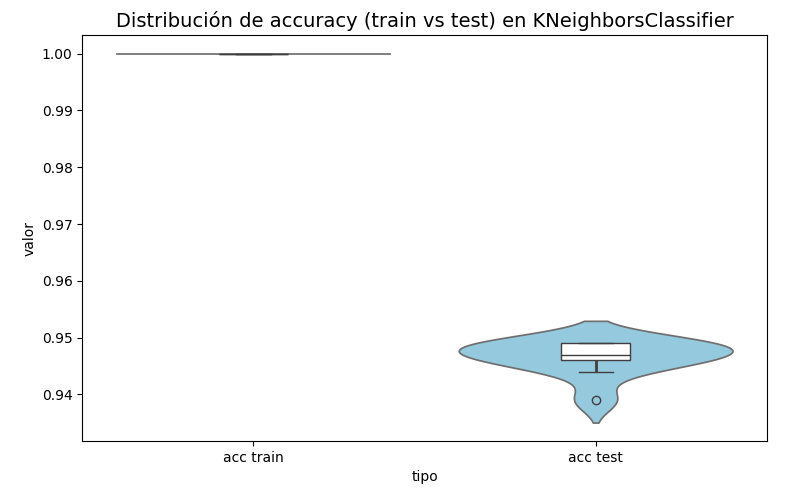
\includegraphics[width=1\linewidth]{Imagenes/knn_bin}
	\caption[\texttt{Boxplot} con \texttt{violinplot} para \textit{K-NN}]{\texttt{Boxplot} con \texttt{violinplot} para \textit{K-NN}.}
	\label{fig:knn_bin}
\end{figure}

\begin{figure}[H]
	\begin{subfigure}{.5\textwidth}
		\centering
		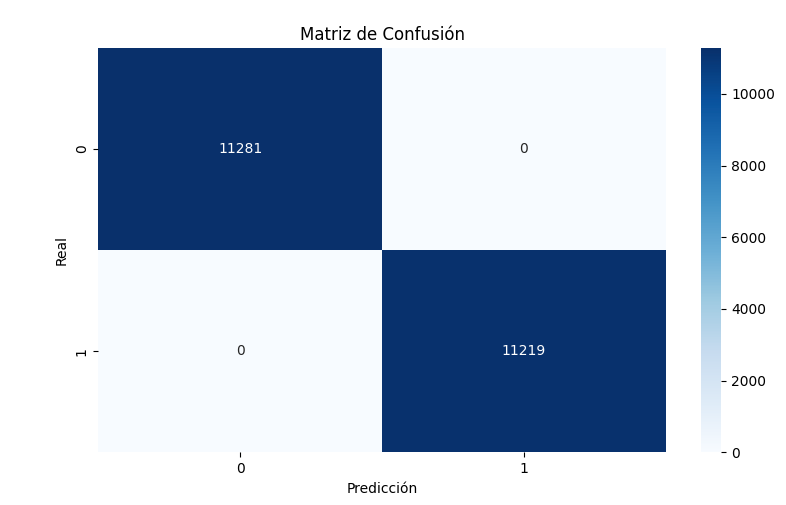
\includegraphics[width=1\linewidth]{Imagenes/knn_bin_mat_train}
		\caption{Matriz de confusión del entrenamiento en la primera semilla.}
		\label{fig:sub-first}
	\end{subfigure}
	\begin{subfigure}{.5\textwidth}
		\centering
		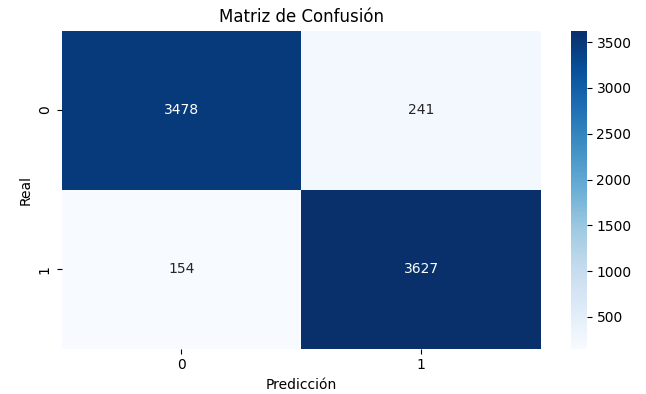
\includegraphics[width=1\linewidth]{Imagenes/knn_bin_mat_test}
		\caption{Matriz de confusión de la generalización en la primera semilla.}
		\label{fig:sub-second}
	\end{subfigure}
	\caption[Matriz de confusión en \textit{K-NN}]{Matriz de confusión en \textit{K-NN}.}
	\label{figT:knn_mat}
\end{figure}

\newpage
\subsection{Máquinas de vectores de soporte}
\label{subsec:svm_bin}

En la tabla \ref{fig:svm_bin} podemos ver cómo para el conjunto de entrenamiento, la precisión se mantiene en valores cercanos a 0.76 en todas las ejecuciones, mientras que (\textit{MS}) muestra variaciones entre 0.656 y 0.704.

\vspace{1em}

En el conjunto de generalización, todas las métricas presentan unos resultados muy similares a los de entrenamiento. Esto se puede apreciar claramente observando la desviación estándar (STD), que indica una baja variabilidad en todas las métricas.

\begin{table}[H]
	\centering
	\begin{tabular}{ |c|c|c|c|c| }
		\hline
		\rowcolor{LightCyan}
		 & \multicolumn{2}{c|}{Entrenamiento} & \multicolumn{2}{c|}{Generalización} \\
		\hline
		\rowcolor{LightCyan}
		 Semilla & Acc & MS & Acc & MS \\
		\hline
		0    & 0.757          & 0.656          & 0.764          & 0.672          \\
		1    & 0.761          & 0.671          & \textbf{0.769} & 0.681          \\
		2    & 0.766          & 0.702          & 0.757          & 0.699          \\
		3    & 0.762          & 0.700          & 0.766          & \textbf{0.704} \\
		4    & 0.760          & 0.684          & 0.768          & 0.696          \\
		5    & 0.761          & 0.663          & 0.753          & 0.655          \\
		6    & 0.762          & 0.702          & 0.762          & 0.683          \\
		7    & 0.763          & 0.699          & 0.759          & 0.697          \\
		8    & \textbf{0.766} & \textbf{0.704} & 0.758          & 0.693          \\
		9    & 0.760          & 0.662          & 0.758          & 0.666          \\
		Mean & 0.762          & 0.684          & 0.762          & 0.685          \\
		STD  & 0.003          & 0.020          & 0.005          & 0.016          \\
		\hline
	\end{tabular}
	\caption{Resultados en entrenamiento y generalización para las distintas semillas en clasificación binaria con \texttt{SVC}.}
	\label{tabla:svm_bin}
\end{table}

Se muestran valores muy consistentes tanto en el conjunto de entrenamiento como en el de test. En la figura \ref{fig:svm_bin}, las distribuciones para ambos conjuntos aparecen concentradas en torno al 0.76, sin grandes variaciones entre diferentes semillas. Esto queda reforzado por la baja dispersión que se observa en el \texttt{boxplot} y por la forma compacta del \texttt{violinplot}, que refleja que no existen valores extremos significativos.

\vspace{1em}

Aunque no se han obtenido los mejores resultados con las máquinas de vectores de soporte, es interesante la estabilidad que consiguen a la hora de generalizar. Esta cercanía entre ambas distribuciones indica que el modelo mantiene un rendimiento estable al generalizar sobre datos no vistos.

\begin{figure}[H]
	\centering
	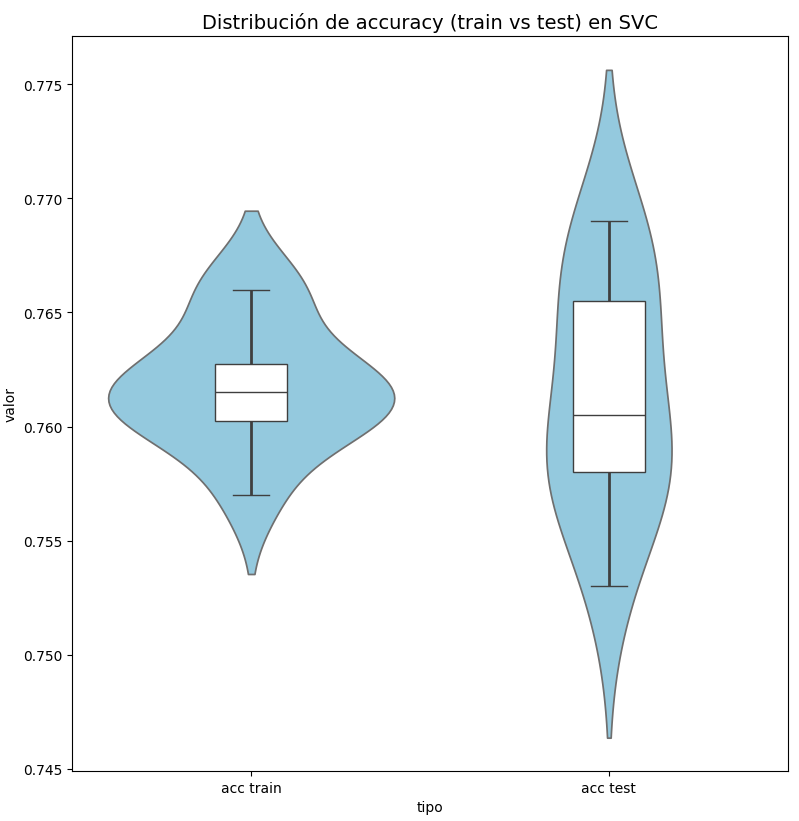
\includegraphics[width=1\linewidth]{Imagenes/svm_bin}
	\caption[\texttt{Boxplot} con \texttt{violinplot} para \textit{SVC}]{\texttt{Boxplot} con \texttt{violinplot} para \textit{SVC}.}
	\label{fig:svm_bin}
\end{figure}

\newpage
\subsection{\textit{Ridge}}
\label{subsec:ridge_bin}

En los resultados obtenidos con el clasificador \texttt{RidgeClassifier}, las métricas de entrenamiento muestran valores estables. La precisión se mantiene en un rango estrecho entre 0.645 y 0.652, con una media de 0.649 y una desviación estándar de 0.002. La mínima sensibilidad presenta mayor variabilidad, con valores comprendidos entre 0.549 y 0.573, alcanzando una media de 0.564 y una desviación estándar de 0.008.

\vspace{1em}

En el conjunto de generalización, la precisión presenta una media de 0.648, muy próxima a la de entrenamiento, y oscila entre 0.639 y 0.655, con una desviación estándar de 0.005. La mínima sensibilidad alcanza una media de 0.561, con valores entre 0.530 y 0.573 y una desviación estándar de 0.014.

\begin{table}[H]
	\centering
	\begin{tabular}{ |c|c|c|c|c| }
		\hline
		\rowcolor{LightCyan}
		 & \multicolumn{2}{c|}{Entrenamiento} & \multicolumn{2}{c|}{Generalización} \\
		\hline
		\rowcolor{LightCyan}
		 Semilla & Acc & MS & Acc & MS \\
		\hline
		0    & 0.649          & 0.549          & 0.648          & 0.530          \\
		1    & 0.645          & 0.558          & \textbf{0.655} & 0.569          \\
		2    & \textbf{0.652} & \textbf{0.573} & 0.645          & 0.564          \\
		3    & 0.649          & 0.567          & 0.653          & 0.570          \\
		4    & 0.651          & 0.573          & 0.651          & \textbf{0.573} \\
		5    & 0.647          & 0.562          & 0.648          & 0.558          \\
		6    & 0.648          & 0.556          & 0.650          & 0.573          \\
		7    & 0.651          & 0.571          & 0.650          & 0.573          \\
		8    & 0.651          & 0.564          & 0.639          & 0.551          \\
		9    & 0.650          & 0.563          & 0.645          & 0.551          \\
		Mean & 0.649          & 0.564          & 0.648          & 0.561          \\
		STD  & 0.002          & 0.008          & 0.005          & 0.014          \\
		\hline
	\end{tabular}
	\caption{Resultados en entrenamiento y generalización para las distintas semillas en clasificación binaria con \texttt{RidgeClassifier}.}
	\label{tabla:ridge_bin}
\end{table}

En la figura \ref{fig:ridge_bin}, se observa que ambos conjuntos presentan valores muy próximos. Las cajas muestran una dispersión reducida, con rangos estrechos tanto en entrenamiento como en test. Esto se traduce en que el modelo ofrece resultados consistentes sin grandes fluctuaciones entre diferentes semillas.

\vspace{1em}

La forma del \texttt{violinplot} refleja estabilidad en el rendimiento, con pequeñas variaciones entre ejecuciones.

\begin{figure}[H]
	\centering
	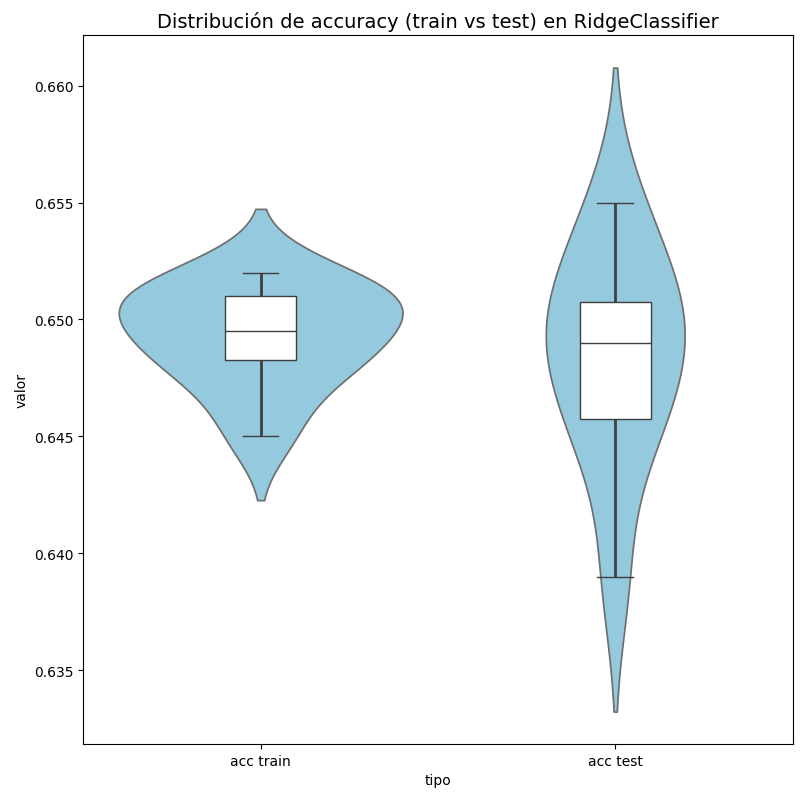
\includegraphics[width=1\linewidth]{Imagenes/ridge_bin}
	\caption[\texttt{Boxplot} con \texttt{violinplot} para \texttt{RidgeClassifier}]{\texttt{Boxplot} con \texttt{violinplot} para \texttt{RidgeClassifier}.}
	\label{fig:ridge_bin}
\end{figure}

\newpage
\subsection{Perceptrón multicapa}
\label{subsec:mlp_bin}

En la tabla \ref{tabla:mlp_bin} se muestran los valores de precisión y mínima sensibilidad tanto en entrenamiento como en generalización para las distintas semillas utilizadas.

\begin{table}[H]
	\centering
	\begin{tabular}{ |c|c|c|c|c| }
		\hline
		\rowcolor{LightCyan}
		 & \multicolumn{2}{c|}{Entrenamiento} & \multicolumn{2}{c|}{Generalización} \\
		\hline
		\rowcolor{LightCyan}
		 Semilla & Acc & MS & Acc & MS \\
		\hline
		0    & 0.783          & 0.771          & 0.789          & 0.778          \\
		1    & 0.788          & 0.736          & \textbf{0.792} & 0.740          \\
		2    & 0.788          & 0.750          & 0.782          & 0.739          \\
		3    & 0.733          & 0.605          & 0.737          & 0.609          \\
		4    & 0.767          & 0.759          & 0.769          & 0.760          \\
		5    & \textbf{0.790} & 0.736          & 0.783          & 0.730          \\
		6    & 0.777          & \textbf{0.772} & 0.783          & \textbf{0.781} \\
		7    & 0.774          & 0.767          & 0.770          & 0.763          \\
		8    & 0.778          & 0.704          & 0.772          & 0.705          \\
		9    & 0.788          & 0.762          & 0.784          & 0.751          \\
		Mean & 0.776          & 0.736          & 0.776          & 0.736          \\
		STD  & 0.017          & 0.051          & 0.016          & 0.050          \\
		\hline
	\end{tabular}
	\caption{Resultados en entrenamiento y generalización para las distintas semillas en clasificación binaria con \texttt{MLPClassifier}.}
	\label{tabla:mlp_bin}
\end{table}

Los resultados de \textit{accuracy} en entrenamiento oscilan entre 0.733 y 0.790, mientras que en generalización se sitúan entre 0.737 y 0.792.

\vspace{1em}

En cuanto a MS, los valores en entrenamiento varían desde 0.605 hasta 0.772, y en generalización desde 0.609 hasta 0.781.

\vspace{1em}

La fila de medias muestra que tanto en entrenamiento como en generalización los promedios de Acc y MS coinciden en 0.776 y 0.736, respectivamente. Las desviaciones típicas reflejan mayor variabilidad en MS frente a la precisión.

\vspace{1em}

La figura \ref{fig:mlp_bin} muestra la distribución de los valores de precisión en entrenamiento y en generalización para las distintas semillas utilizadas.

\begin{figure}[H]
	\centering
	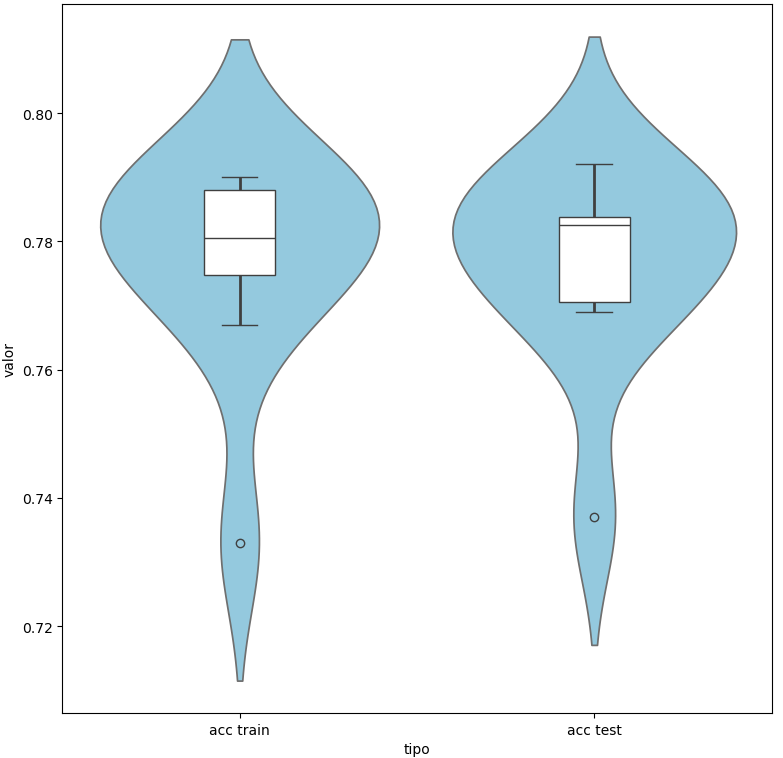
\includegraphics[width=1\linewidth]{Imagenes/mlp_bin}
	\caption[\texttt{Boxplot} con \texttt{violinplot} para \texttt{MLPClassifier}]{\texttt{Boxplot} con \texttt{violinplot} para \texttt{MLPClassifier}.}
	\label{fig:mlp_bin}
\end{figure}

En entrenamiento, la caja es relativamente compacta, aunque se observa un valor que queda por debajo de la mayoría de las mediciones. Este caso podría considerarse ruido, pero sería necesaria una muestra de resultados mayor para poder asegurarlo.

\vspace{1em}

En generalización, la distribución es muy similar, con valores que oscilan entre 0.73 y 0.79 y una mediana también próxima a 0.78. La dispersión es comparable a la observada en el entrenamiento, mostrando que los resultados se mantienen consistentes entre ambos conjuntos.

\vspace{1em}

El \texttt{violinplot} refleja que en ambas situaciones la densidad principal se concentra en torno a la franja de 0.77–0.79, indicando que la mayoría de ejecuciones producen resultados en ese rango.

\subsection{\textit{Light gradient boosting machine}}
\label{subsec:lgbm_bin}

Los valores de precisión y mínima sensibilidad obtenidos en entrenamiento y generalización para las distintas semillas se muestran en la tabla \ref{tabla:lgbm_bin}

\begin{table}[H]
	\centering
	\begin{tabular}{ |c|c|c|c|c| }
		\hline
		\rowcolor{LightCyan}
		 & \multicolumn{2}{c|}{Entrenamiento} & \multicolumn{2}{c|}{Generalización} \\
		\hline
		\rowcolor{LightCyan}
		 Semilla & Acc & MS & Acc & MS \\
		\hline
		0    & 0.984          & 0.981          & 0.953          & \textbf{0.952} \\
		1    & 0.984          & 0.980          & 0.951          & 0.947          \\
		2    & 0.985          & 0.983          & 0.949          & 0.946          \\
		3    & 0.985          & 0.982          & 0.952          & 0.951          \\
		4    & 0.984          & 0.981          & 0.950          & 0.945          \\
		5    & 0.985          & 0.981          & 0.949          & 0.948          \\
		6    & 0.985          & 0.982          & 0.952          & 0.949          \\
		7    & 0.986          & 0.984          & 0.948          & 0.947          \\
		8    & 0.984          & 0.979          & 0.953          & 0.952          \\
		9    & \textbf{0.989} & \textbf{0.989} & \textbf{0.953} & 0.950          \\
		Mean & 0.985          & 0.982          & 0.951          & 0.949          \\
		STD  & 0.002          & 0.003          & 0.002          & 0.002          \\
		\hline
	\end{tabular}
	\caption{Resultados en entrenamiento y generalización para las distintas semillas en clasificación binaria con \texttt{LGBMClassifier}}
	\label{tabla:lgbm_bin}
\end{table}

En el conjunto de entrenamiento, los valores de \textit{accuracy} se sitúan entre 0.984 y 0.989, con una media de 0.985 y una desviación estándar de 0.002. MS toma valores entre 0.979 y 0.989, con una media de 0.982 y desviación estándar de 0.003.

\vspace{1em}

En generalización, la precisión oscila entre 0.948 y 0.953, con una media de 0.951 y desviación estándar de 0.002. Para MS, los resultados están entre 0.945 y 0.952, con una media de 0.949 y desviación estándar de 0.002.

\begin{figure}[H]
	\centering
	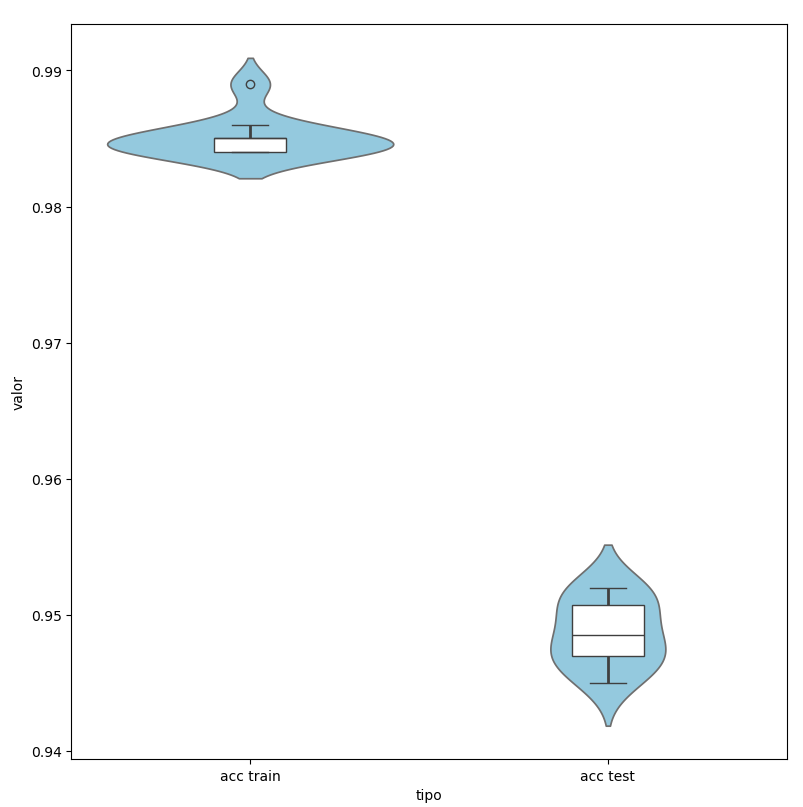
\includegraphics[width=1\linewidth]{Imagenes/lgbm_bin}
	\caption[\texttt{Boxplot} con \texttt{violinplot} para \texttt{LGBMClassifier}]{\texttt{Boxplot} con \texttt{violinplot} para \texttt{LGBMClassifier}.}
	\label{fig:lgbm_bin}
\end{figure}

En la figura \ref{fig:lgbm_bin}, vemos que el modelo muestra un rendimiento muy consistente, con distribución de precisión estrecha y centrada en torno a valores elevados tanto en entrenamiento como en generalización. La cercanía de ambas distribuciones indica que no existe un sobreajuste significativo, ya que el comportamiento en entrenamiento y en test es muy similar.

\newpage
Además, la baja dispersión en las métricas sugiere que el modelo es estable frente a las distintas semillas de inicialización, lo que respalda su fiabilidad al aplicarse en diferentes ejecuciones. En general, se trata de un modelo robusto, con buen equilibrio entre ajuste a los datos de entrenamiento y capacidad de generalización.

\subsection{Discusión de los resultados}
\label{subsec:discusion}

Las tablas \ref{tabla:resumen_modelos} y \ref{tabla:resumen_std}, resumen los valores medios y las desviaciones típicas de las métricas Acc y MS en entrenamiento y generalización para los distintos modelos implementados.

En la tabla \ref{tabla:resumen_modelos}, se observa que varios modelos alcanzan valores altos y consistentes de precisión, con pequeñas variaciones entre entrenamiento y generalización. Sin embargo, existen diferencias notables en la estabilidad de la métrica de mínima sensibilidad, lo que permite distinguir entre metodologías más o menos equilibradas a la hora de clasificar correctamente todas las clases.

\begin{table}[H]
	\centering
	\begin{tabular}{|c|c|c|c|c|}
		\hline
		\rowcolor{LightCyan}
		Modelo & \multicolumn{2}{c|}{Entrenamiento} & \multicolumn{2}{c|}{Generalización} \\
		\hline
		\rowcolor{LightCyan}
		Clasificador & Acc & MS & Acc & MS \\
		\hline
		\texttt{DecisionTreeClassifier} & 0.981 & 0.931 & 0.939 & 0.501 \\
		\texttt{RandomForestClassifier} & 0.981 & 0.931 & 0.939 & 0.501 \\
		\texttt{KNeighborsClassifier}   & 1.000 & 1.000 & 0.947 & 0.934 \\
		\texttt{SVC}                    & 0.762 & 0.684 & 0.762 & 0.685 \\
		\texttt{RidgeClassifier}        & 0.649 & 0.564 & 0.648 & 0.561 \\
		\texttt{MLPClassifier}          & 0.776 & 0.736 & 0.776 & 0.736 \\
		\texttt{LGBMClassifier}         & 0.985 & 0.982 & 0.951 & 0.949 \\
		\hline
	\end{tabular}
	\caption{Resumen de resultados medios en entrenamiento y generalización para cada modelo}
	\label{tabla:resumen_modelos}
\end{table}

La tabla \ref{tabla:resumen_std} refleja la variabilidad de los resultados frente al uso de diferentes semillas de inicialización. Mientras que algunos modelos poca variación, otros presentan una dispersión algo más elevada, especialmente en la métrica de mínima sensibilidad, lo que señala una mayor dependencia de la partición de datos y menor consistencia en la clasificación.

\begin{table}[H]
	\centering
	\begin{tabular}{|c|c|c|c|c|}
		\hline
		\rowcolor{LightCyan}
		Modelo & \multicolumn{2}{c|}{Entrenamiento} & \multicolumn{2}{c|}{Generalización} \\
		\hline
		\rowcolor{LightCyan}
		& Acc & MS & Acc & MS \\
		\hline
		\texttt{DecisionTreeClassifier} & 0.004 & 0.016 & 0.014 & 0.016 \\
		\texttt{RandomForestClassifier} & 0.004 & 0.016 & 0.014 & 0.016 \\
		\texttt{KNeighborsClassifier}   & 0.000 & 0.000 & 0.003 & 0.004 \\
		\texttt{SVC}                    & 0.003 & 0.020 & 0.005 & 0.016 \\
		\texttt{RidgeClassifier}        & 0.002 & 0.008 & 0.005 & 0.014 \\
		\texttt{MLPClassifier}          & 0.017 & 0.051 & 0.016 & 0.050 \\
		\texttt{LGBMClassifier}         & 0.002 & 0.003 & 0.002 & 0.002 \\
		\hline
	\end{tabular}
	\caption{Resumen de desviaciones típicas en entrenamiento y generalización para cada modelo}
	\label{tabla:resumen_std}
\end{table}

Observando estos resultados, podemos destacar ligeramente las siguientes metodologías:

\begin{itemize}
	\item \texttt{LGBMClassifier}: Presenta valores medios muy elevados en entrenamiento y en generalización y sus desviaciones típicas son mínimas, lo que demuestra alta estabilidad y consistencia. Es un modelo con gran capacidad de generalización y muy bajo riesgo de sobreajuste.
	\item \texttt{KNeighborsClassifier}: Obtiene resultados muy altos y equilibrados entre entrenamiento y generalización y sus desviaciones típicas son extremadamente bajas, con comportamiento muy estable. Aunque no alcanza los valores máximos absolutos de otros métodos, la estabilidad y consistencia lo convierten en una opción muy competitiva.
\end{itemize}

En la gráfica representada en la figura \ref{fig:vs_bin} podemos ver que entre estas dos opciones, el clasificador \texttt{LGBMClassifier} obtiene un rendimiento ligeramente superior.

\begin{figure}[H]
	\centering
	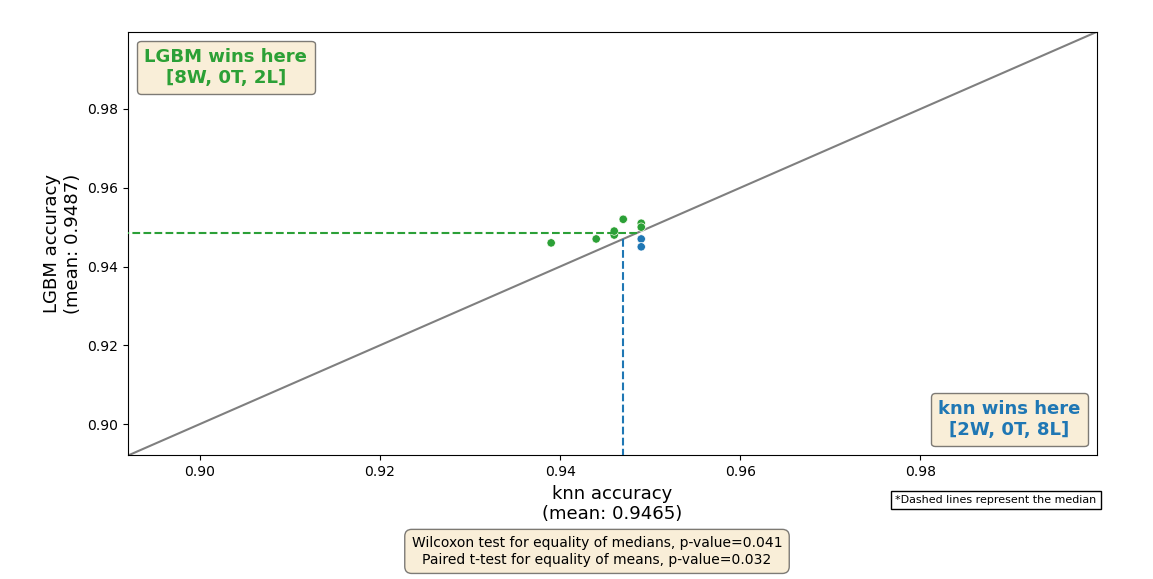
\includegraphics[width=1\linewidth]{Imagenes/vs_bin}
	\caption[Comparativa entre los modelos \texttt{KNegihborsClassifier} y \texttt{LGBMClassifier}]{Comparativa entre los modelos \texttt{KNegihborsClassifier} y \texttt{LGBMClassifier}.}
	\label{fig:vs_bin}
\end{figure}

\newpage
\section{Clasificación multiclase}
\label{sec:clas_multi}

A continuación se comentarán los resultados de los diferentes modelos para tener una visión general de como se comportan en la clasificación multiclase disponible en nuestro conjunto de datos.

\subsection{Árboles de decisión}
\label{subsec:dt_multi}

En la tabla \ref{tabla:dt_multi} se muestran los valores de accuracy y mínima sensibilidad.

\begin{table}[H]
	\centering
	\begin{tabular}{ |c|c|c|c|c| }
		\hline
		\rowcolor{LightCyan}
		 & \multicolumn{2}{c|}{Entrenamiento} & \multicolumn{2}{c|}{Generalización} \\
		\hline
		\rowcolor{LightCyan}
		 Estado aleatorio & Acc & MS & Acc & MS \\
		\hline
		0    & 0.980          & 0.928          & 0.939          & 0.524          \\
		1    & 0.980          & 0.929          & 0.939          & 0.500          \\
		2    & 0.980          & 0.927          & \textbf{0.941} & 0.429          \\
		3    & 0.979          & 0.923          & 0.939          & 0.444          \\
		4    & 0.982          & 0.931          & 0.939          & 0.500          \\
		5    & 0.980          & 0.929          & 0.937          & \textbf{0.609} \\
		6    & 0.978          & 0.920          & 0.938          & 0.550          \\
		7    & 0.980          & 0.929          & 0.939          & 0.562          \\
		8    & 0.982          & 0.934          & 0.938          & 0.489          \\
		9    & \textbf{0.989} & \textbf{0.956} & 0.936          & 0.400          \\
		Mean & 0.981          & 0.931          & 0.939          & 0.501          \\
		STD  & 0.003          & 0.010          & 0.001          & 0.064          \\
		\hline
	\end{tabular}
	\caption{Resultados en entrenamiento y generalización para las distintas semillas en clasificación binaria con  \texttt{DecisionTreeClassifier}.}
	\label{tabla:dt_multi}
\end{table}

La precisión en entrenamiento oscila entre 0.978 y 0.989, mientras que en test se sitúan entre 0.936 y 0.941. En cuanto a mínima sensibilidad, los valores en entrenamiento varían desde 0.920 hasta 0.956, y en test desde 0.400 hasta 0.609.

\vspace{1em}

Los promedios de \textit{accuracy} son 0.981 en entrenamiento y 0.939 en test, mientras que los promedios de MS son 0.931 en entrenamiento y 0.501 en test.

\begin{figure}[H]
	\centering
	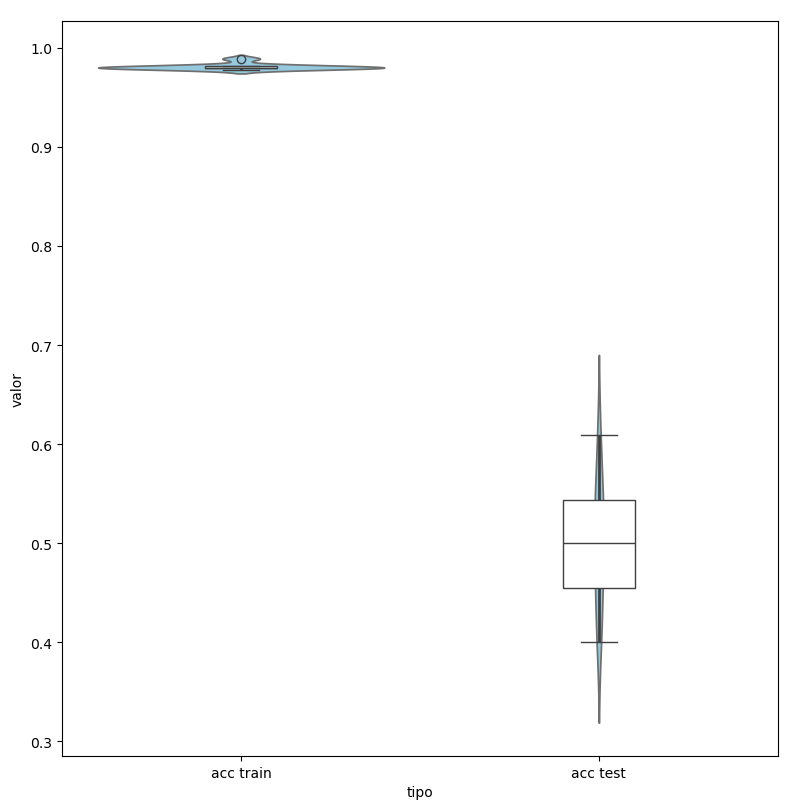
\includegraphics[width=1\linewidth]{Imagenes/dt_multi}
	\caption[\texttt{Boxplot} con \texttt{violinplot} para árboles de decisión en clasificación multiclase]{\texttt{Boxplot} con \texttt{violinplot} para árboles de decisión en clasificación multiclase.}
	\label{fig:dt_multi}
\end{figure}

En la figura \ref{fig:dt_multi} vemos como el modelo muestra un comportamiento consistente, con distribuciones relativamente concentradas en torno a valores altos tanto en entrenamiento como en test. Las formas de los \texttt{violinplot} indican que la mayoría de las ejecuciones se agrupan cerca de la mediana, con pocas variaciones extremas.

\vspace{1em}

La comparación entre las distribuciones de entrenamiento y test refleja que las métricas de generalización se mantienen cercanas a las de entrenamiento, lo que sugiere estabilidad en el rendimiento del modelo. La dispersión reducida también indica que los resultados son poco sensibles a la elección de la semilla, lo que respalda la fiabilidad del modelo en distintas ejecuciones. En conjunto, se observa un modelo equilibrado y robusto, con buen ajuste a los datos y capacidad de generalización.

\vspace{1em}

Por otro lado, en los resultados de la tabla \ref{tabla:dt_multi}, apreciamos una caída significativa entre los resultados de MS en entrenamiento y generalización, lo que puede indicar ciertos problemas a la hora de clasificar patrones no conocidos.

\subsection{\textit{Random forest}}
\label{subsec:rf_multi}

En la tabla \ref{tabla:rf_multi} se observan los resultados obtenidos para cada semilla de inicialización en entrenamiento y test.

\begin{table}[H]
	\centering
	\begin{tabular}{ |c|c|c|c|c| }
		\hline
		\rowcolor{LightCyan}
		 & \multicolumn{2}{c|}{Entrenamiento} & \multicolumn{2}{c|}{Generalización} \\
		\hline
		\rowcolor{LightCyan}
		 Estado aleatorio & Acc & MS & Acc & MS \\
		\hline
		0    & 0.981          & 0.926          & 0.951          & 0.524          \\
		1    & 0.981          & 0.926          & 0.953          & \textbf{0.735} \\
		2    & 0.981          & 0.926          & 0.954          & 0.429          \\
		3    & 0.980          & 0.923          & 0.954          & 0.500          \\
		4    & 0.981          & 0.926          & \textbf{0.954} & 0.500          \\
		5    & \textbf{0.981} & \textbf{0.927} & 0.952          & 0.638          \\
		6    & 0.980          & 0.923          & 0.952          & 0.550          \\
		7    & 0.981          & 0.927          & 0.954          & 0.500          \\
		8    & 0.981          & 0.926          & 0.953          & 0.471          \\
		9    & 0.981          & 0.926          & 0.953          & 0.400          \\
		Mean & 0.981          & 0.926          & 0.953          & 0.525          \\
		STD  & 0.000          & 0.002          & 0.001          & 0.098          \\
		\hline
	\end{tabular}
	\caption{Resultados en entrenamiento y generalización para las distintas semillas en clasificación multiclase con  \texttt{RandomForestClassifier}.}
	\label{tabla:rf_multi}
\end{table}

Los valores de accuracy se mantienen altos y consistentes en entrenamiento, con una media de 0.981 y desviación estándar muy baja (0.000), indicando un comportamiento uniforme entre las diferentes ejecuciones. La mínima sensibilidad muestra cierta variabilidad entre semillas, con valores que oscilan y una desviación estándar de 0.002 en entrenamiento.

\vspace{1em}

En los datos de test, el Acc promedio es de 0.953, con desviación estándar de 0.001, mientras que la mínima sensibilidad presenta una mayor dispersión (STD = 0.098).

\begin{figure}[H]
	\centering
	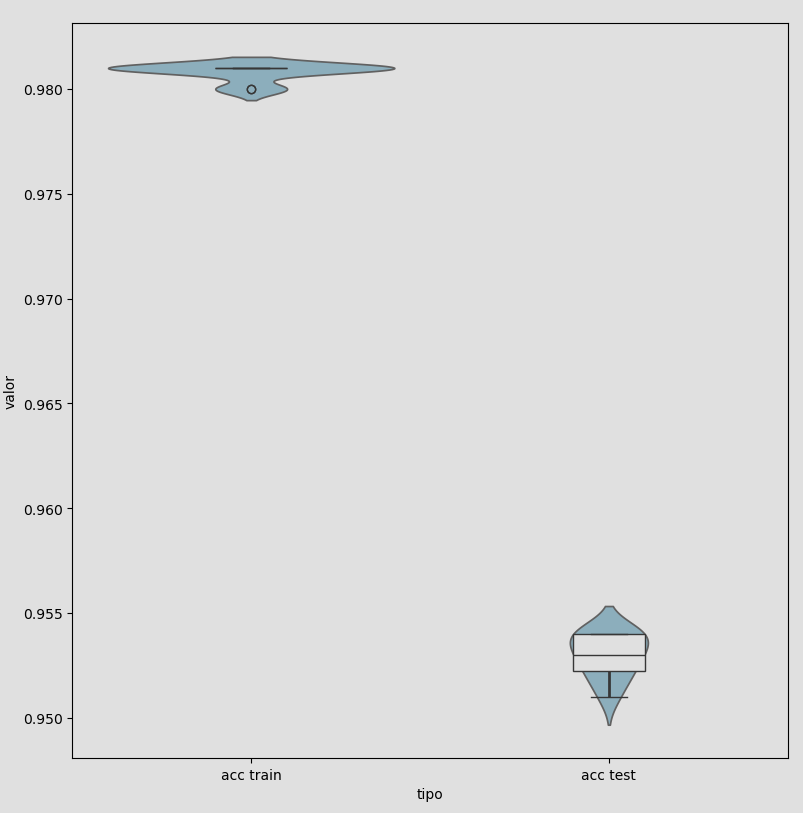
\includegraphics[width=1\linewidth]{Imagenes/rf_multi}
	\caption[\texttt{Boxplot} con \texttt{violinplot} para \texttt{RandomForestClassifier} en clasificación multiclase]{\texttt{Boxplot} con \texttt{violinplot} para \texttt{RandomForestClassifier} en clasificación multiclase.}
	\label{fig:rf_multi}
\end{figure}

El modelo presenta un desempeño elevado en \textit{accuracy}, con valores de entrenamiento muy estables y prácticamente constantes en todas las ejecuciones. En la figura \ref{fig:rf_multi}, la distribución de los resultados de entrenamiento se concentra de forma marcada en torno a un mismo valor, sin apenas dispersión.

\vspace{1em}

En los datos de test, la precisión se sitúa próxima a la de entrenamiento, con un ligero descenso que se mantiene consistente en todas las semillas. La forma del \texttt{violinplot} refleja poca variabilidad, y el \texttt{boxplot} confirma que la mediana y los cuartiles se encuentran muy próximos entre sí.

\vspace{1em}

En conjunto, el comportamiento sugiere un modelo que mantiene estabilidad entre entrenamiento y generalización, pero no asegura un comportamiento homogéneo por clases: la MS en test es más baja e inestable, lo que apunta a dificultades para recuperar consistentemente las clases más difíciles.

\subsection{\textit{K-NN}}
\label{subsec:knn_multi}


En la tabla \ref{tabla:knn_multi}, podemos ver como en el entrenamiento, la métrica Acc se mantiene constante en 0.994 en todos los casos, mientras que MS varía entre 0.794 y 0.849. En el conjunto de prueba, Acc oscila entre 0.939 y 0.943, y MS presenta valores comprendidos entre 0.357 y 0.529.

\vspace{1em}

Para la media, tenemos un Acc de 0.994 y un MS de 0.815 en entrenamiento, y un Acc de 0.941 junto a un MS de 0.451 en prueba. Por su parte, las desviaciones estándar en entrenamiento son de 0.000 para Acc y 0.016 para MS, mientras que en prueba alcanzan 0.001 para Acc y 0.067 para MS.
\begin{table}[H]
	\centering
	\begin{tabular}{ |c|c|c|c|c| }
		\hline
		\rowcolor{LightCyan}
		 & \multicolumn{2}{c|}{Entrenamiento} & \multicolumn{2}{c|}{Generalización} \\
		\hline
		\rowcolor{LightCyan}
		 Estado aleatorio & Acc & MS & Acc & MS \\
		\hline
		0    & 0.994          & 0.811          & 0.940          & 0.524          \\
		1    & 0.994          & 0.794          & \textbf{0.943} & 0.500          \\
		2    & 0.994          & 0.811          & 0.940          & 0.357          \\
		3    & 0.994          & 0.815          & 0.942          & 0.389          \\
		4    & 0.994          & 0.810          & 0.941          & 0.375          \\
		5    & 0.994          & 0.807          & 0.940          & 0.435          \\
		6    & 0.994          & 0.802          & 0.941          & 0.500          \\
		7    & \textbf{0.994} & \textbf{0.849} & 0.940          & 0.500          \\
		8    & 0.994          & 0.817          & 0.939          & \textbf{0.529} \\
		9    & 0.994          & 0.834          & 0.940          & 0.400          \\
		Mean & 0.994          & 0.815          & 0.941          & 0.451          \\
		STD  & 0.000          & 0.016          & 0.001          & 0.067          \\
		\hline
	\end{tabular}
	\caption{Resultados en entrenamiento y generalización para las distintas semillas en clasificación multiclase con \texttt{KNeighborsClassifier}.}
	\label{tabla:knn_multi}
\end{table}

Los resultados muestran que el modelo obtiene un rendimiento muy alto y estable en el conjunto de entrenamiento y un valor de MS cercano a 0.815 en promedio, con muy poca variación. Esto indica que el modelo se ajusta de forma consistente a los datos de entrenamiento.

\vspace{1em}

En el conjunto de prueba, la exactitud también es elevada aunque más baja, pero con estabilidad. Sin embargo, el MS presenta valores más bajos y con mayor dispersión.

\vspace{1em}

En conjunto, el modelo es consistente es precisión, aunque la métrica MS indica que existen diferencias en cómo se comporta según la partición de los datos. Como MS es más alto y estable en entrenamiento, esto podría indicar que el modelo se ajusta muy bien a los datos de entrenamiento, pero al enfrentarse a datos no vistos pierde algo de consistencia.

\newpage
\subsection{Máquinas de vectores de soporte}
\label{subsec:svm_multi}

En este caso, el proceso de entrenamiento presentó una mayor complejidad y dificultad para obtener resultados comparables con los de otros modelos evaluados, principalmente debido a las limitaciones del equipo utilizado. El elevado tiempo requerido para el entrenamiento sin ajuste de parámetros, junto con los resultados poco satisfactorios obtenidos para las dos semillas empleadas ---con una precisión aproximada del 20\%---, motivaron la decisión de no continuar con las máquinas de vectores de soporte para la clasificación multiclase. No obstante, estos resultados no indican que el modelo sea inadecuado para el problema planteado, sino que tiene una mayor exigencia en cuanto a los recursos necesarios para su entrenamiento.

\subsection{\textit{Ridge}}
\label{subsec:ridge_multi}

La tabla \ref{tabla:ridge_multi} muestra los resultados de \texttt{RidgeClassifier} en diez ejecuciones con distintos estados aleatorios.

\vspace{1em}

La Precisión en entrenamiento varía entre 0.170 y 0.195, con un promedio de 0.182 y una desviación estándar de 0.009 mientras que en prueba fluctúa entre 0.166 y 0.191, con promedio 0.182 y desviación estándar 0.009.La métrica MS es 0.000 en todas las ejecuciones, tanto para entrenamiento como para prueba.

\vspace{1em}

A pesar de que hay estabilidad y capacidad de generalización en el modelo, los resultados son extremadamente pobres. Estos resultados pueden atribuirse a la naturaleza lineal del RidgeClassifier, que limita su capacidad para adaptarse a problemas de alta complejidad o con relaciones no lineales entre las características como puede ser el caso del \textit{malware}.

\begin{table}[H]
	\centering
	\begin{tabular}{ |c|c|c|c|c| }
		\hline
		\rowcolor{LightCyan}
		 & \multicolumn{2}{c|}{Entrenamiento} & \multicolumn{2}{c|}{Generalización} \\
		\hline
		\rowcolor{LightCyan}
		 Estado aleatorio & Acc & MS & Acc & MS \\
		\hline
		0    & 0.189          & 0.000          & 0.186          & 0.000          \\
		1    & \textbf{0.195} & \textbf{0.000} & \textbf{0.191} & \textbf{0.000} \\
		2    & 0.173          & 0.000          & 0.176          & 0.000          \\
		3    & 0.172          & 0.000          & 0.172          & 0.000          \\
		4    & 0.185          & 0.000          & 0.189          & 0.000          \\
		5    & 0.187          & 0.000          & 0.189          & 0.000          \\
		6    & 0.170          & 0.000          & 0.166          & 0.000          \\
		7    & 0.186          & 0.000          & 0.191          & 0.000          \\
		8    & 0.187          & 0.000          & 0.187          & 0.000          \\
		9    & 0.171          & 0.000          & 0.173          & 0.000          \\
		Mean & 0.182          & 0.000          & 0.182          & 0.000          \\
		STD  & 0.009          & 0.000          & 0.009          & 0.000          \\
		\hline
	\end{tabular}
	\caption{Resultados en entrenamiento y generalización para las distintas semillas en clasificación multiclase con \texttt{RidgeClassifier}}
	\label{tabla:ridge_multi}
\end{table}

\newpage
\subsection{Perceptrón multicapa}
\label{subsec:mlp_multi}

En la tabla \ref{tabla:mlp_multi} vemos como la precisión en entrenamiento varía entre 0.679 y 0.730, con promedio de 0.717 y desviación estándar de 0.014, mientras que en generalización oscila entre 0.681 y 0.735, con promedio de 0.718 y desviación estándar de 0.014.

\begin{table}[H]
	\centering
	\begin{tabular}{ |c|c|c|c|c| }
		\hline
		\rowcolor{LightCyan}
		 & \multicolumn{2}{c|}{Entrenamiento} & \multicolumn{2}{c|}{Generalización} \\
		\hline
		\rowcolor{LightCyan}
		 Estado aleatorio & Acc & MS & Acc & MS \\
		\hline
		0    & 0.725          & 0.000          & 0.722          & 0.000          \\
		1    & 0.724          & 0.000          & 0.724          & 0.000          \\
		2    & 0.724          & 0.000          & 0.723          & 0.000          \\
		3    & 0.679          & 0.000          & 0.681          & 0.000          \\
		4    & \textbf{0.730} & \textbf{0.000} & \textbf{0.735} & \textbf{0.000} \\
		5    & 0.721          & 0.000          & 0.717          & 0.000          \\
		6    & 0.724          & 0.000          & 0.723          & 0.000          \\
		7    & 0.711          & 0.000          & 0.711          & 0.000          \\
		8    & 0.719          & 0.000          & 0.720          & 0.000          \\
		9    & 0.716          & 0.000          & 0.718          & 0.000          \\
		Mean & 0.717          & 0.000          & 0.718          & 0.000          \\
		STD  & 0.014          & 0.000          & 0.014          & 0.000          \\
		\hline
	\end{tabular}
	\caption{Resultados en entrenamiento y generalización para las distintas semillas en clasificación multiclase con \texttt{MLPClassifier}}
	\label{tabla:mlp_multi}
\end{table}

El modelo muestra un rendimiento consistente y relativamente alto en precisión, como podemos ver en el gráfico representado en la figura \ref{fig:mlp_multi}, tanto en entrenamiento como en prueba, lo que indica estabilidad y buena capacidad de generalización. A pesar de esto, la métrica MS se mantiene en cero, lo que evidencia que el modelo no logra capturar completamente la diversidad de clases ni ciertos patrones específicos del conjunto de datos. La cercanía entre el desempeño en entrenamiento y prueba sugiere que no existe sobreajuste significativo; sin embargo, las limitaciones en MS reflejan que el modelo todavía enfrenta dificultades para manejar todos los aspectos del problema multiclase, posiblemente debido la la cantidad de clases con pocos patrones.

\begin{figure}[H]
	\centering
	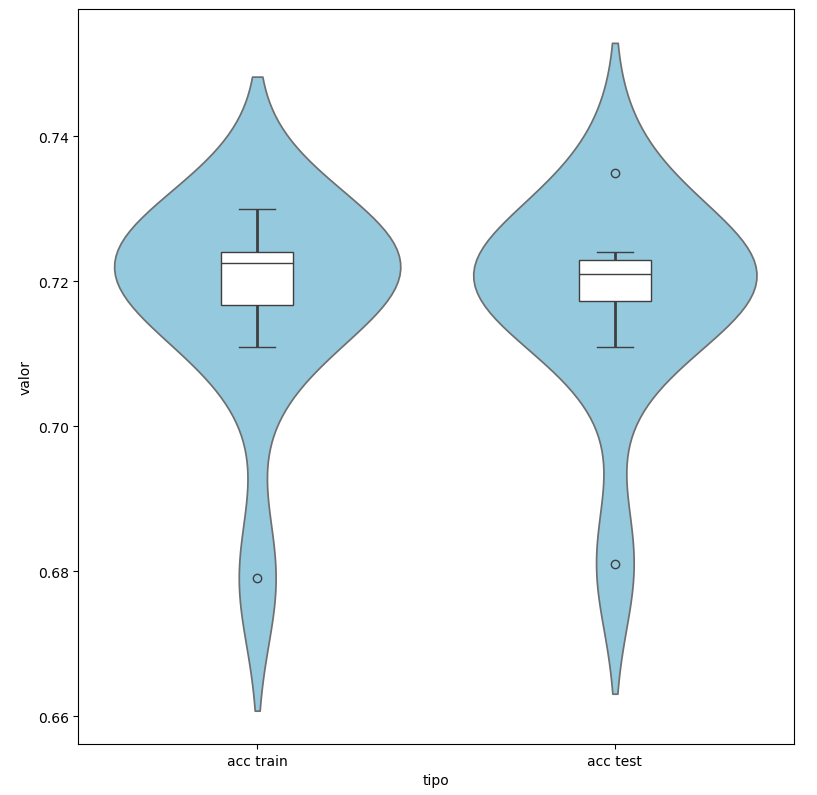
\includegraphics[width=1\linewidth]{Imagenes/mlp_multi}
	\caption[\texttt{Boxplot} con \texttt{violinplot} para \texttt{MLPClassifier} en clasificación multiclase]{\texttt{Boxplot} con \texttt{violinplot} para \texttt{MLPClassifier} en clasificación multiclase.}
	\label{fig:mlp_multi}
\end{figure}

\newpage
\subsection{\textit{Light gradient boosting machine}}
\label{subsec:lgbm_multi}

La tabla \ref{tabla:lgbm_multi}, muestra los resultados de precisión y mínima sensibilidad \texttt{LGBMClassifier} en diez ejecuciones con distintos estados aleatorios.

\begin{table}[H]
	\centering
	\begin{tabular}{ |c|c|c|c|c|c| }
		\hline
		\rowcolor{LightCyan}
		 & \multicolumn{2}{c|}{Entrenamiento} & \multicolumn{2}{c|}{Test} \\
		\hline
		\rowcolor{LightCyan}
		 Estado aleatorio & Acc & MS & Acc & MS \\
		\hline
		0    & 0.938          & 0.821          & 0.916          & 0.600          \\
		1    & 0.936          & 0.820          & 0.916          & \textbf{0.735} \\
		2    & 0.890          & 0.749          & 0.884          & 0.357          \\
		3    & 0.323          & 0.000          & 0.327          & 0.000          \\
		4    & 0.888          & 0.747          & 0.880          & 0.500          \\
		5    & \textbf{0.938} & \textbf{0.828} & \textbf{0.917} & 0.565          \\
		6    & 0.893          & 0.758          & 0.881          & 0.550          \\
		7    & 0.936          & 0.821          & 0.917          & 0.562          \\
		8    & 0.891          & 0.750          & 0.880          & 0.588          \\
		9    & 0.893          & 0.760          & 0.883          & 0.467          \\
		Mean & 0.853          & 0.706          & 0.840          & 0.492          \\
		STD  & 0.187          & 0.250          & 0.181          & 0.198          \\
		\hline
	\end{tabular}
	\caption{Resultados en entrenamiento y generalización para las distintas semillas en clasificación multiclase con \texttt{LGBMClassifier}}
	\label{tabla:lgbm_multi}
\end{table}

El Acc en entrenamiento presenta valores muy variables entre ejecuciones, mientras que en prueba también se observa variabilidad, aunque ligeramente menor. La mínima sensibilizad en entrenamiento y prueba oscila entre valores altos y cero, reflejando diferencias importantes entre ejecuciones. La desviación típica de todas las métricas es bastante alta, situándose en 0.25 para MS en entrenamiento.

\begin{figure}[H]
	\centering
	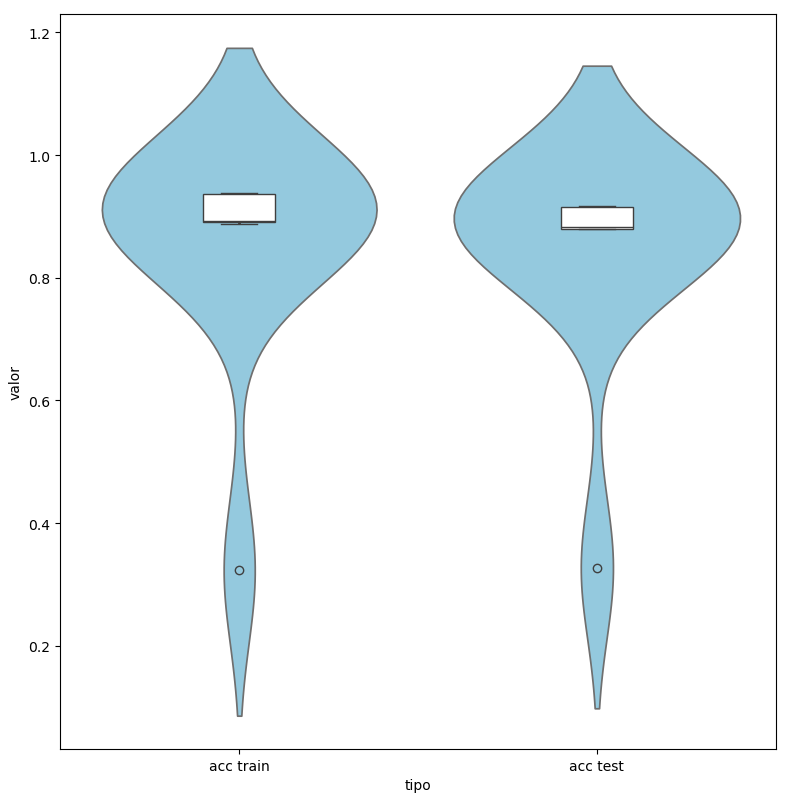
\includegraphics[width=1\linewidth]{Imagenes/lgbm_multi}
	\caption[\texttt{Boxplot} con \texttt{violinplot} para \texttt{LGBMClassifier} en clasificación multiclase]{\texttt{Boxplot} con \texttt{violinplot} para \texttt{LGBMClassifier} en clasificación multiclase.}
	\label{fig:lgbm_multi}
\end{figure}

Como podemos ver en la figura \ref{fig:lgbm_multi}, este modelo muestra un rendimiento alto y relativamente consistente en la mayoría de ejecuciones, tanto en entrenamiento como en prueba. La excepción corresponde a una ejecución aislada, que podría considerarse ruido en una muestra mayor, cuyos resultados están muy por debajo del resto. Podemos interpretar que no representa el comportamiento típico del modelo.

\vspace{1em}

Si no tenemos en cuenta esta muestra, el modelo tiene buena generalización, además de estabilidad entre entrenamiento y prueba, aunque algunas diferencias menores sugieren que puede haber un ligero sobreajuste. La métrica MS indica que el modelo no captura de manera uniforme todos los patrones de las clases.

\subsection{Discusión de los resultados}
\label{subsec:discusion_multi}

Las tablas \ref{tabla:resumen_mean} y \ref{tabla:resumen_std}, resumen los valores medios y las desviaciones típicas de las métricas Acc y MS en entrenamiento y generalización para los distintos modelos implementados.

\vspace{1em}

En la tabla \ref{tabla:resumen_mean} se presentan las medias de las métricas de exactitud y mínima sensibilidad tanto en entrenamiento como en generalización para cada modelo. Se observa que algunos modelos alcanzan valores altos y consistentes de exactitud en ambas fases, mientras que otros presentan valores notablemente más bajos, especialmente en mínima sensibilidad. Esta información permite comparar el rendimiento promedio de cada metodología y proporciona una visión general de cuáles modelos tienden a clasificar correctamente todas las clases de manera más equilibrada.

\begin{table}[H]
	\centering
	\begin{tabular}{|c|c|c|c|c|}
		\hline
		\rowcolor{LightCyan}
		Modelo & \multicolumn{2}{c|}{Entrenamiento} & \multicolumn{2}{c|}{Generalización} \\
		\hline
		\rowcolor{LightCyan}
		& Acc & MS & Acc & MS \\
		\hline
		\texttt{KNeighborsClassifier}   & 0.994 & 0.815 & 0.941 & 0.451 \\
		\texttt{RidgeClassifier}        & 0.182 & 0.000 & 0.182 & 0.000 \\
		\texttt{MLPClassifier}          & 0.717 & 0.000 & 0.718 & 0.000 \\
		\texttt{LGBMClassifier}         & 0.853 & 0.706 & 0.840 & 0.492 \\
		\texttt{DecisionTreeClassifier} & 0.981 & 0.931 & 0.939 & 0.501 \\
		\texttt{RandomForestClassifier} & 0.981 & 0.926 & 0.953 & 0.525 \\
		\texttt{SVC}                    & --    & --    & --    & --    \\
		\hline
	\end{tabular}
	\caption{Resumen de medias de métricas en entrenamiento y generalización para cada modelo}
	\label{tabla:resumen_mean}
\end{table}

\newpage
En la tabla \ref{tabla:resumen_std_multi} se muestran las desviaciones estándar de las métricas de exactitud y mínima sensibilidad. Algunos modelos presentan desviaciones muy bajas, reflejando consistencia y uniformidad en sus resultados, mientras que otros muestran variaciones más altas, especialmente en mínima sensibilidad. Estos datos permiten identificar qué modelos son más confiables, así como aquellos cuya capacidad de predicción puede depender de la semilla o partición de los datos.

\begin{table}[H]
	\centering
	\begin{tabular}{|c|c|c|c|c|}
		\hline
		\rowcolor{LightCyan}
		Modelo & \multicolumn{2}{c|}{Entrenamiento} & \multicolumn{2}{c|}{Generalización} \\
		\hline
		\rowcolor{LightCyan}
		& Acc & MS & Acc & MS \\
		\hline
		\texttt{KNeighborsClassifier}   & 0.000 & 0.016 & 0.001 & 0.067 \\
		\texttt{RidgeClassifier}        & 0.009 & 0.000 & 0.009 & 0.000 \\
		\texttt{MLPClassifier}          & 0.014 & 0.000 & 0.014 & 0.000 \\
		\texttt{LGBMClassifier}         & 0.187 & 0.250 & 0.181 & 0.198 \\
		\texttt{DecisionTreeClassifier} & 0.003 & 0.010 & 0.001 & 0.064 \\
		\texttt{RandomForestClassifier} & 0.000 & 0.002 & 0.001 & 0.098 \\
		\texttt{SVC}                    & --    & --    & --    & --    \\
		\hline
	\end{tabular}
	\caption{Resumen de desviaciones típicas en entrenamiento y generalización para cada modelo}
	\label{tabla:resumen_std_multi}
\end{table}

Analizando todos los modelos evaluados, se observa que el \texttt{RandomForestClassifier} y el \texttt{KNeighborsClassifier} son los que presentan el mejor rendimiento. El primero de ellos destaca por su alta precisión y mínima sensibilidad tanto en entrenamiento como en generalización, con desviaciones estándar bajas, lo que indica resultados consistentes y confiables. El segundo, muestra también una exactitud elevada y resultados estables, con una mínima sensibilidad aceptable. Aunque su MS es ligeramente inferior a la de RandomForest, mantiene un buen equilibrio entre rendimiento y consistencia

\vspace{1em}

En la gráfica representada en la figura \ref{fig:vs_multi} podemos ver que entre estas dos opciones, el clasificador \texttt{RandomForestClassifier} obtiene un rendimiento ligeramente superior.

\begin{figure}[H]
	\centering
	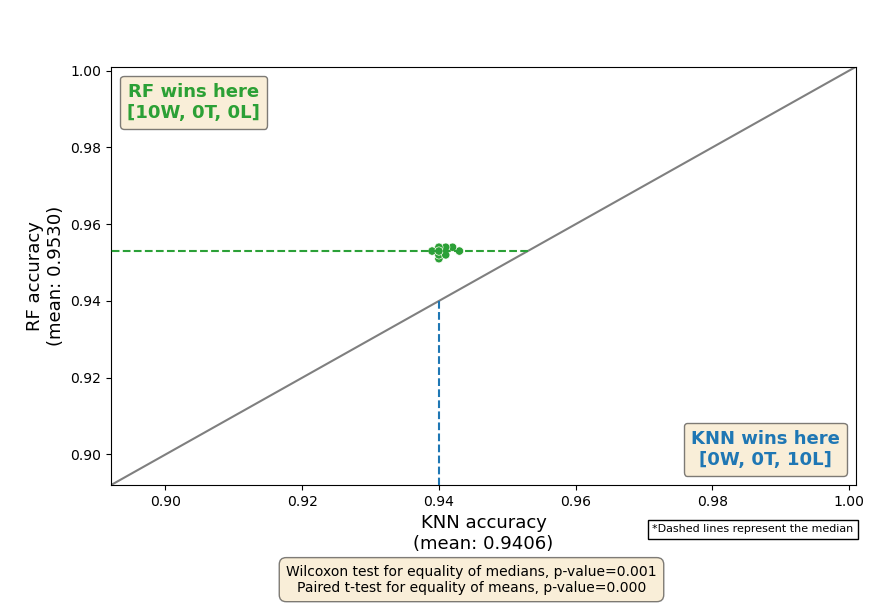
\includegraphics[width=1\linewidth]{Imagenes/vs_multi}
	\caption[Comparativa entre los modelos \texttt{KNegihborsClassifier} y \texttt{LGBMClassifier}]{Comparativa entre los modelos \texttt{KNegihborsClassifier} y \texttt{LGBMClassifier}.}
	\label{fig:vs_multi}
\end{figure}
